\section{Neural Path Framework}\label{sec:npf}
In this section, we extend the \emph{neural path} framework developed by \citetalias{ch2020neural}, to CNN and ResNet architectures described in the previous section. The neural path framework exploits the gating property of ReLU activation, which can be thought of as gate/mask that blocks/allows its pre-activation input depending on its $0/1$ state ( $0$ if pre-activation is negative and $1$ if pre-activation is positive). The key idea here is to  break a DNN (with ReLU) into paths, and express its output as a summation of the contribution of the paths. The contribution of a path is the product of the signal in its input node, the weights in the path and the gates in the path. For a DNN with $P$ paths, for an input $x\in\R^{\din}$,  the gating information is encoded in a novel \emph{neural path feature} (NPF), $\phi_{x,\Theta}\in\R^P$ and a novel \emph{neural path value} (NPV), $v_{\Theta}\in\R^P$ encodes the weights.  The output of the DNN is then the inner product of the NPFs and NPVs, i.e., $\hat{y}_{\Theta}(x_s)=\ip{\phi_{x_s,\Theta},v_{\Theta}}$ (\Cref{prop:zero}).
\begin{definition}
A path starts from an input node, passes through weights, hidden nodes, and normalisation constants and ends at the output node.
\end{definition}
\begin{proposition}
The total number of paths in FC-DNN, CNN and ResNet are respectively given by $\Pfc=\din w^{(d-1)}$,  $\Pcnn=\din(\wconv w)^{\dc}w^{(\dfc-1)}$ and $\Pres = \din \cdot\sum_{i=0}^b \binom{b}{i} w^{(i+2)\dblock-1}$.
\end{proposition}
\begin{notation}[Index Maps]
The ranges of index maps $\Ifeat_l$,  $\Iconv_l$, $\I_l$ are $[\din]$, $[\wconv]$ and $[w]$ respectively. The index maps are used to identify the nodes through which a path $p$ passes. Further, let $\I^{\J}(p)\colon [\Pres]\ra 2^{[b]}$ specify the indices of the skip connections ignored in path $p$.  Also, we follow the convention that weights and gating values of layers corresponding to blocks skipped are $1$.
\end{notation}

\begin{definition}[Path Activity]
The product of the gating values in a path $p$ is its `activity' denoted by $A_{\Theta}(x,p)$. We define:

(a) $A_{\Theta}(x,p)=\Pi_{l=1}^{d-1} G_{x,\Theta}(\I_l(p),l)$, for FC-DNN and ResNet.

(b) $A_{\Theta}(x,p)=\Pi_{l=1}^{\dc+1} G_{x,\Theta}(\Ifeat_l(p),\I_l(p),l)\cdot\Pi_{l=\dc+2}^{\dc+\dfc+1} G_{x,\Theta}(\I_l(p),l)$, for CNN.

In CNN, the pooling layer is accounted by letting $G=G^{\text{pool}}$ for $l=\dc+1$.
\begin{comment}
\emph{
\begin{tabular}{ll}
$A_{\Theta}(x,p)=\Pi_{l=1}^{d-1} G_{x,\Theta}(\I_l(p),l)$& for FC and ResNet\\
$A_{\Theta}(x,p)=\Pi_{l=1}^{\dc} G_{x,\Theta}(\Ifeat_l(p),\I_l(p),l)\cdot G^{\text{pool}}_{x\Theta}(\Ifeat_{\dc+1}(p),\I_{dc+1}(p),\dc+1)\cdot\Pi_{l=\dc+2}^{\dc+\dfc+1} G_{x,\Theta}(\I_l(p),l)$ & for CNN.\\
\end{tabular}
}
\end{comment}
\end{definition}
\begin{comment}
\begin{notation}[Index Map in FC-DNN]
Let $\I_0\colon[P]\ra [\din], \I_{l}\colon [P]\ra [w],l=1,\ldots,d-1, \I_d\colon [P]\ra [1]$ provide the index of the hidden unit through which a path $p$ passes in layer $l$. Further, let $\I^{\J}(p)\colon [\Pres]\ra 2^{[b]}$ specify the indices of the skip connections ignored in path $p$.  Also, we follow the convention that weights and gating values of layers corresponding to blocks skipped are $1$.
\end{notation}
\end{comment}
\begin{comment}
\begin{figure}
\begin{minipage}{0.5\columnwidth}
\begin{tabular}{|l|l|}\hline
Index Map & Layers\\\hline
$\Ifeat_{l}\colon [P]\ra[\din]$ & $l=0$\\\hline
$\Iconv_{l}\colon [P]\ra[\wconv]$ & $l=0,\ldots,\dc$\\\hline
$\Iwidth_{l}\colon [P]\ra[1]$  & $l=0$\\ \hline
$\Iwidth_{l}\colon [P]\ra[w]$  & $l=1,\ldots,\dc+\dfc$\\ \hline
$\Iwidth_{l}\colon [P]\ra[1]$  & $l=\dc+\dfc+1$\\ \hline
\end{tabular}
\end{minipage}
\begin{minipage}{0.5\columnwidth}
\resizebox{\columnwidth}{!}{
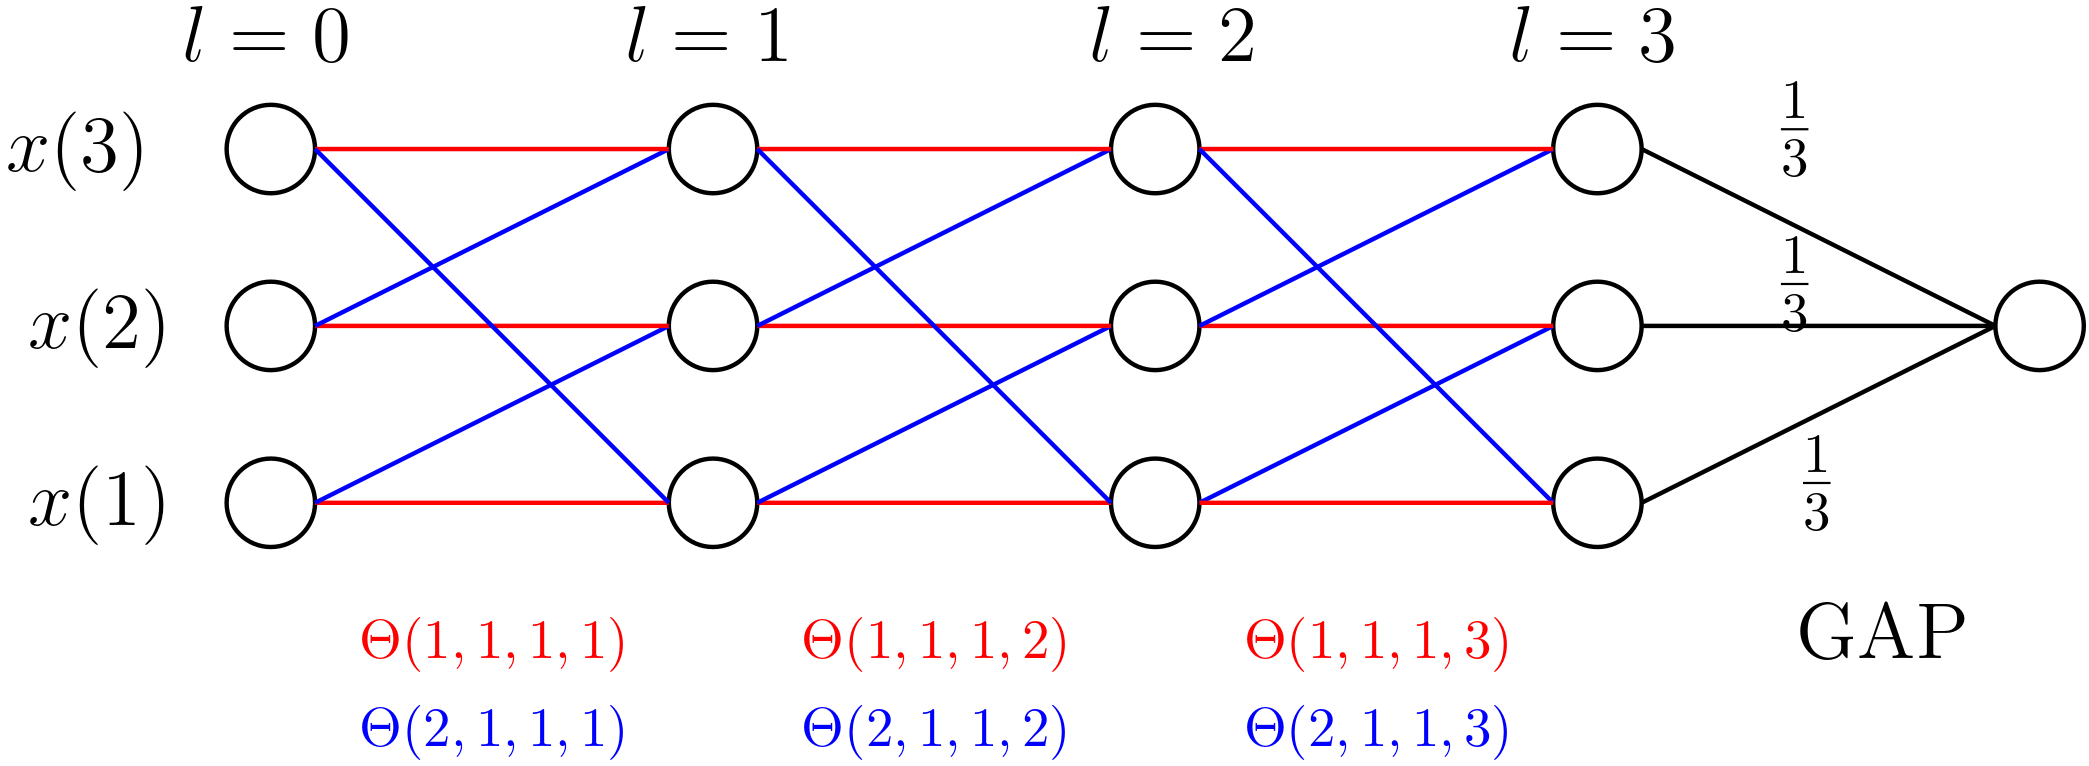
\includegraphics[scale=0.1]{figs/pathshare.png}
}
\end{minipage}
\end{figure}
\end{comment}
\begin{comment}
\begin{notation}[Index Map in ResNet] $\I_0\colon[\Pres]\ra [\din]$, $\I_{l}\colon [\Pres]\ra [w]l=1,\ldots,\dblock, (b+1)\dblock,\ldots,(b+2)\dblock-1$, $\I_{l}\colon [\Pres]\ra [w]\cup\emptyset, l=\dblock+1,\ldots,(b+1)\dblock$. Further, let $\I^{\J}(p)\colon [\Pres]\ra 2^{[b]}$ specify the indices of the skip connections ignored in path $p$. Also, $\emptyset$ denotes an empty index and we follow the convention that weights and gating values through empty indices are $1$.
\end{notation}
\end{comment}
\begin{comment}
\begin{definition}[Index Map in ResNet]
The index maps that specify the weights through which a given path $p$ passes are specified as given below.
\begin{center}
\begin{tabular}{|c|l|}\hline
Index Set & Layer\\\hline
$\I_l\colon[\Pres]\ra [\din]$ & $l=0$\\\hline
$\I_{l}\colon [\Pres]\ra [w]$ &  $l=1,\ldots,\dblock$ and $l=(b+1)\dblock,\ldots,(b+2)\dblock-1$\\\hline
$\I_{l}\colon [\Pres]\ra [w]\cup\emptyset$ &  $l=\dblock+1,\ldots,(b+1)\dblock$\\\hline
\end{tabular}
\end{center}
Further, let $\I^{\J}(p)\colon [\Pres]\ra 2^{[b]}$ specify the indices of the skip connections ignored in path $p$. Also, $\emptyset$ denotes an empty index and we follow the convention that weights and gating values through empty indices are $1$.
\end{definition}
\end{comment}
\begin{definition}[Bundle Paths of Sharing Weights]\label{def:bundle}
Let $\hat{P}^{\text{cnn}}=\frac{\Pcnn}{\din}$, and $\{B_1,\ldots, B_{\hat{P}^{\text{cnn}}}\}$ be a collection of sets such that $\forall i,j\in [\hat{P}^{\text{cnn}}], i\neq j$ we have $B_i\cap B_j=\emptyset$ and $\cup_{i=1}^{\hat{P}^{\text{cnn}}}B_i =[\Pcnn]$. Further,  if paths $p,p' \in B_i$, then $\Iconv_l(p)=\Iconv_l(p'), \forall l=1,\ldots, \dc$ and $\I_l(p)=\I_l(p'), \forall l=0,\ldots, \dc$.
\end{definition}
\begin{proposition}\label{prop:bundle}
There are exactly $\din$ paths in a bundle.
\end{proposition}

\begin{definition}[Normalisation Factor]
Define $\Gamma(\J)\eqdef \underset{j\in J}\Pi \gamma^{\text{pre}}_j \cdot \underset{j'\in [b]}\Pi \gamma^{\text{post}}_{j'}$
\end{definition}
 Weight sharing is shown in the the cartoon in \Cref{fig:pathshare}, which shows a CNN with $\din=3$, $w=1$, $\wconv=2$, $\dc=3$, $\dfc=0$. Here, the red coloured paths all share the same weights  $\Theta(1,1,1,l), l=1,2,3$ and the blue coloured paths all share the same weights given by $\Theta(2,1,1,l), l=1,2,3$. 
\FloatBarrier
 \begin{figure}[h]
\begin{minipage}{0.33\columnwidth}
\resizebox{\columnwidth}{!}{
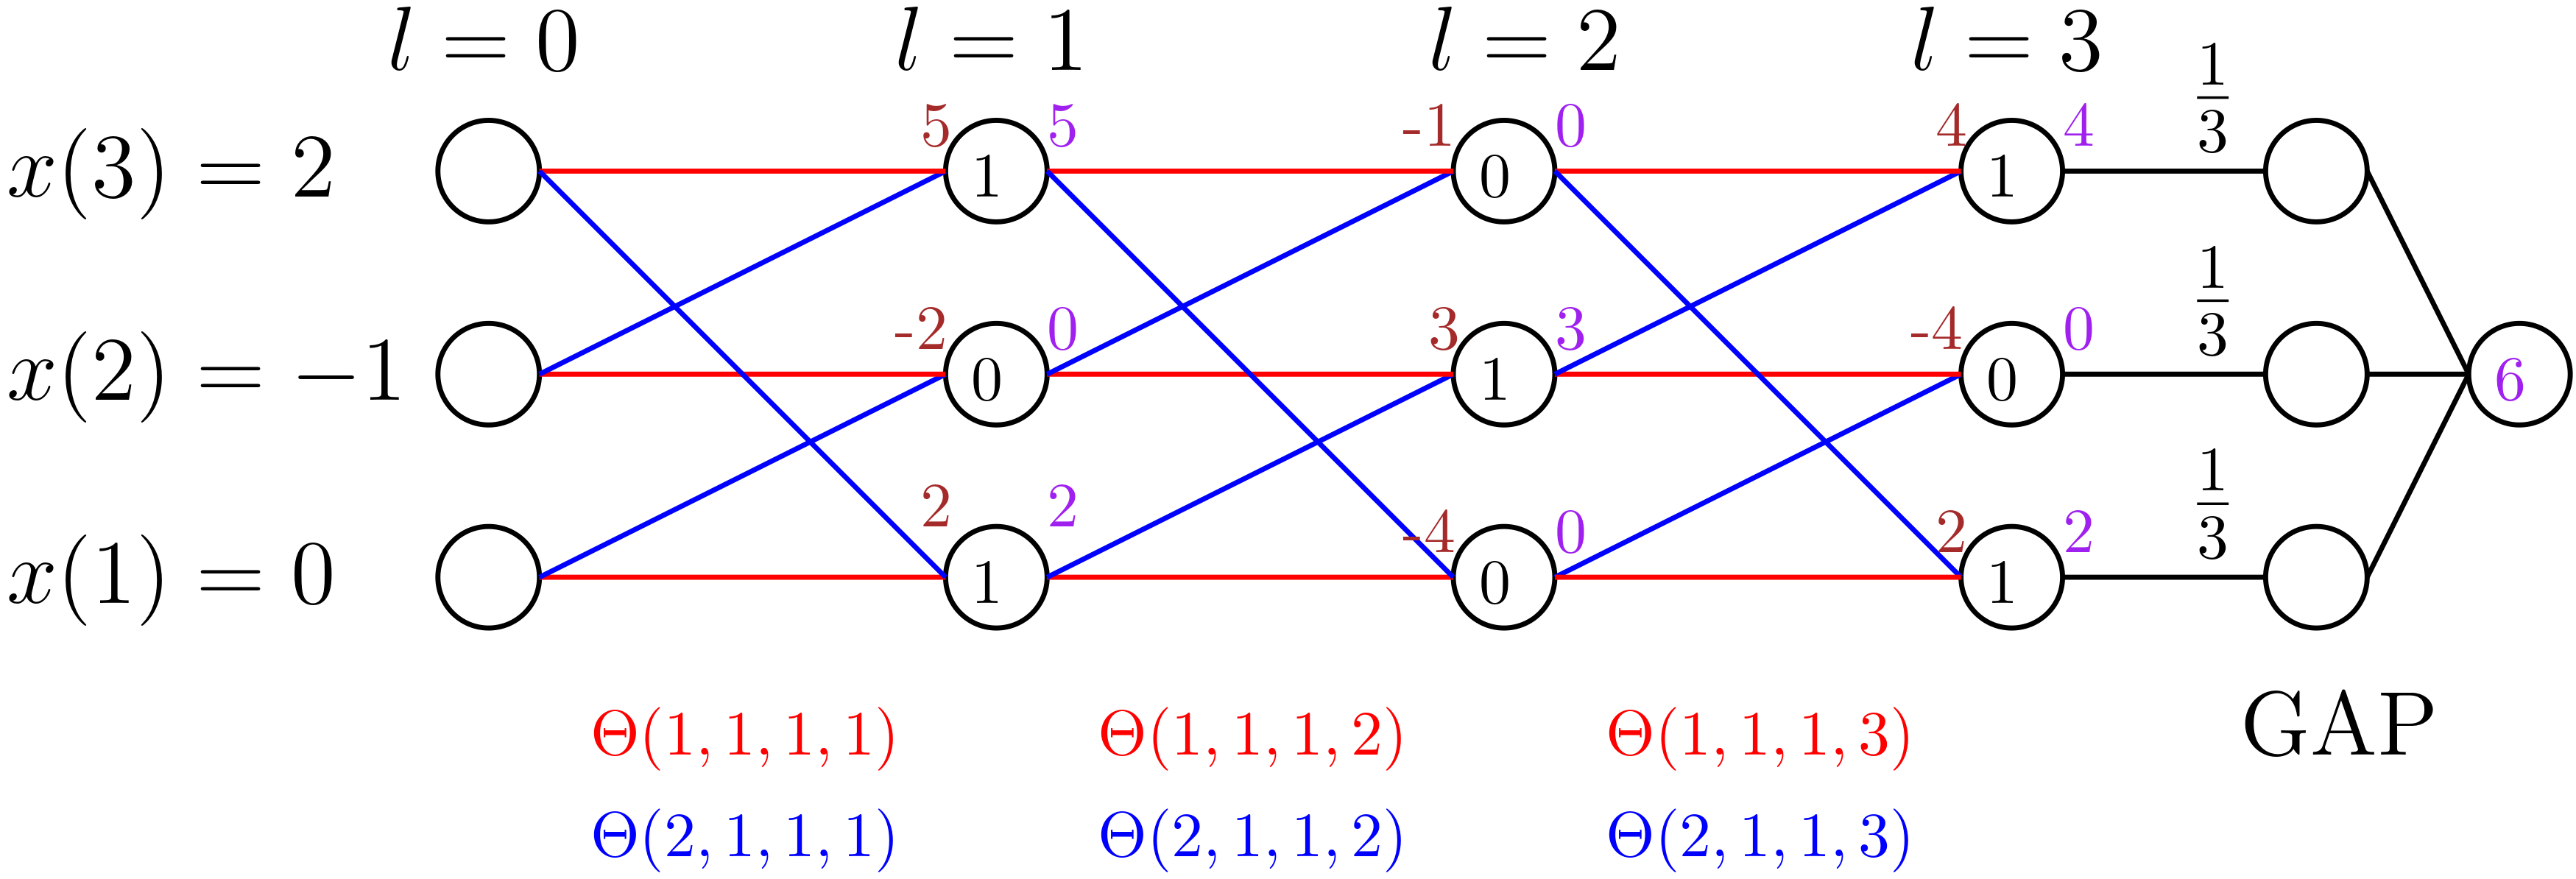
\includegraphics[angle=0.2,scale=0.1]{figs/gap.png}
}
\end{minipage}
\begin{minipage}{0.33\columnwidth}
\resizebox{\columnwidth}{!}{
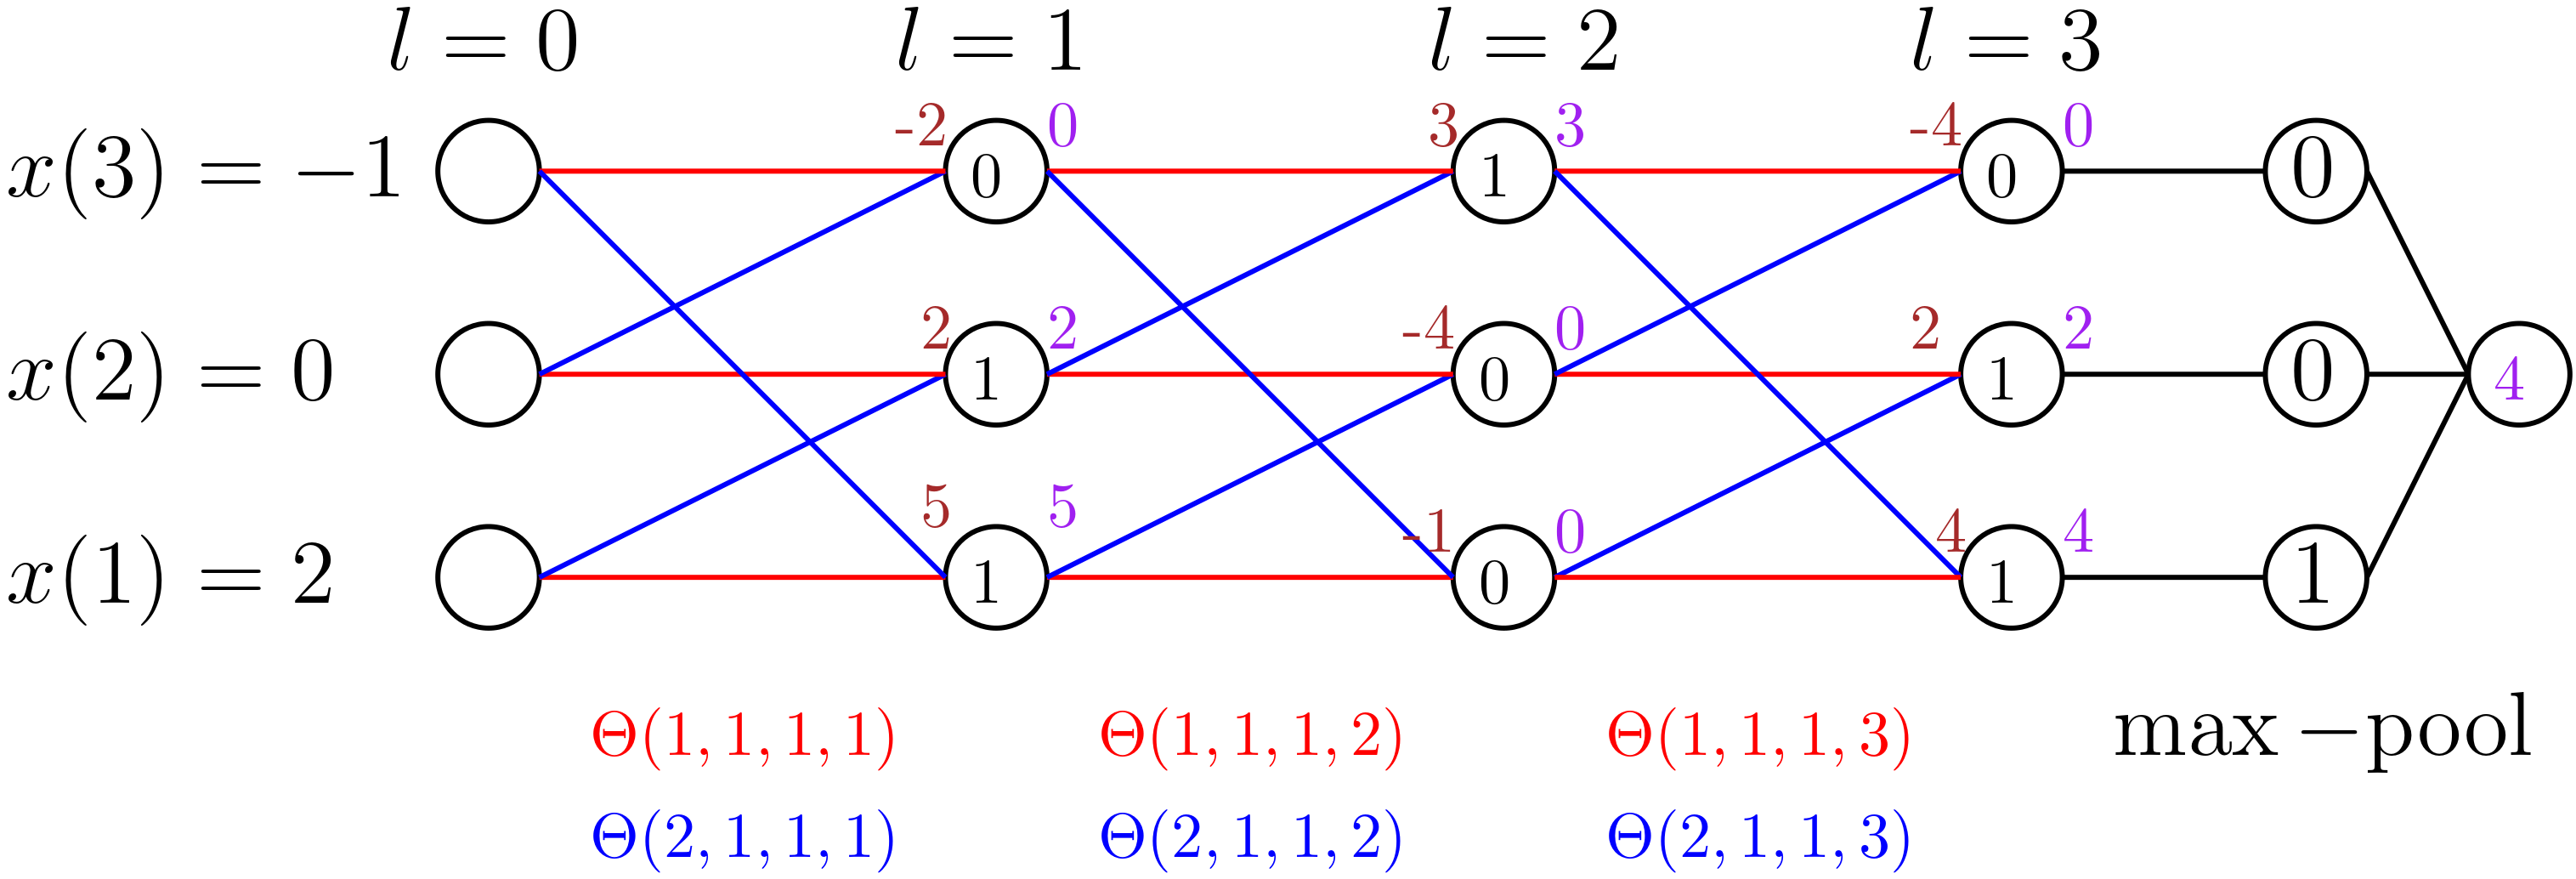
\includegraphics[angle=0.2,scale=0.1]{figs/maxp1.png}
}
\end{minipage}
\begin{minipage}{0.33\columnwidth}
\resizebox{\columnwidth}{!}{
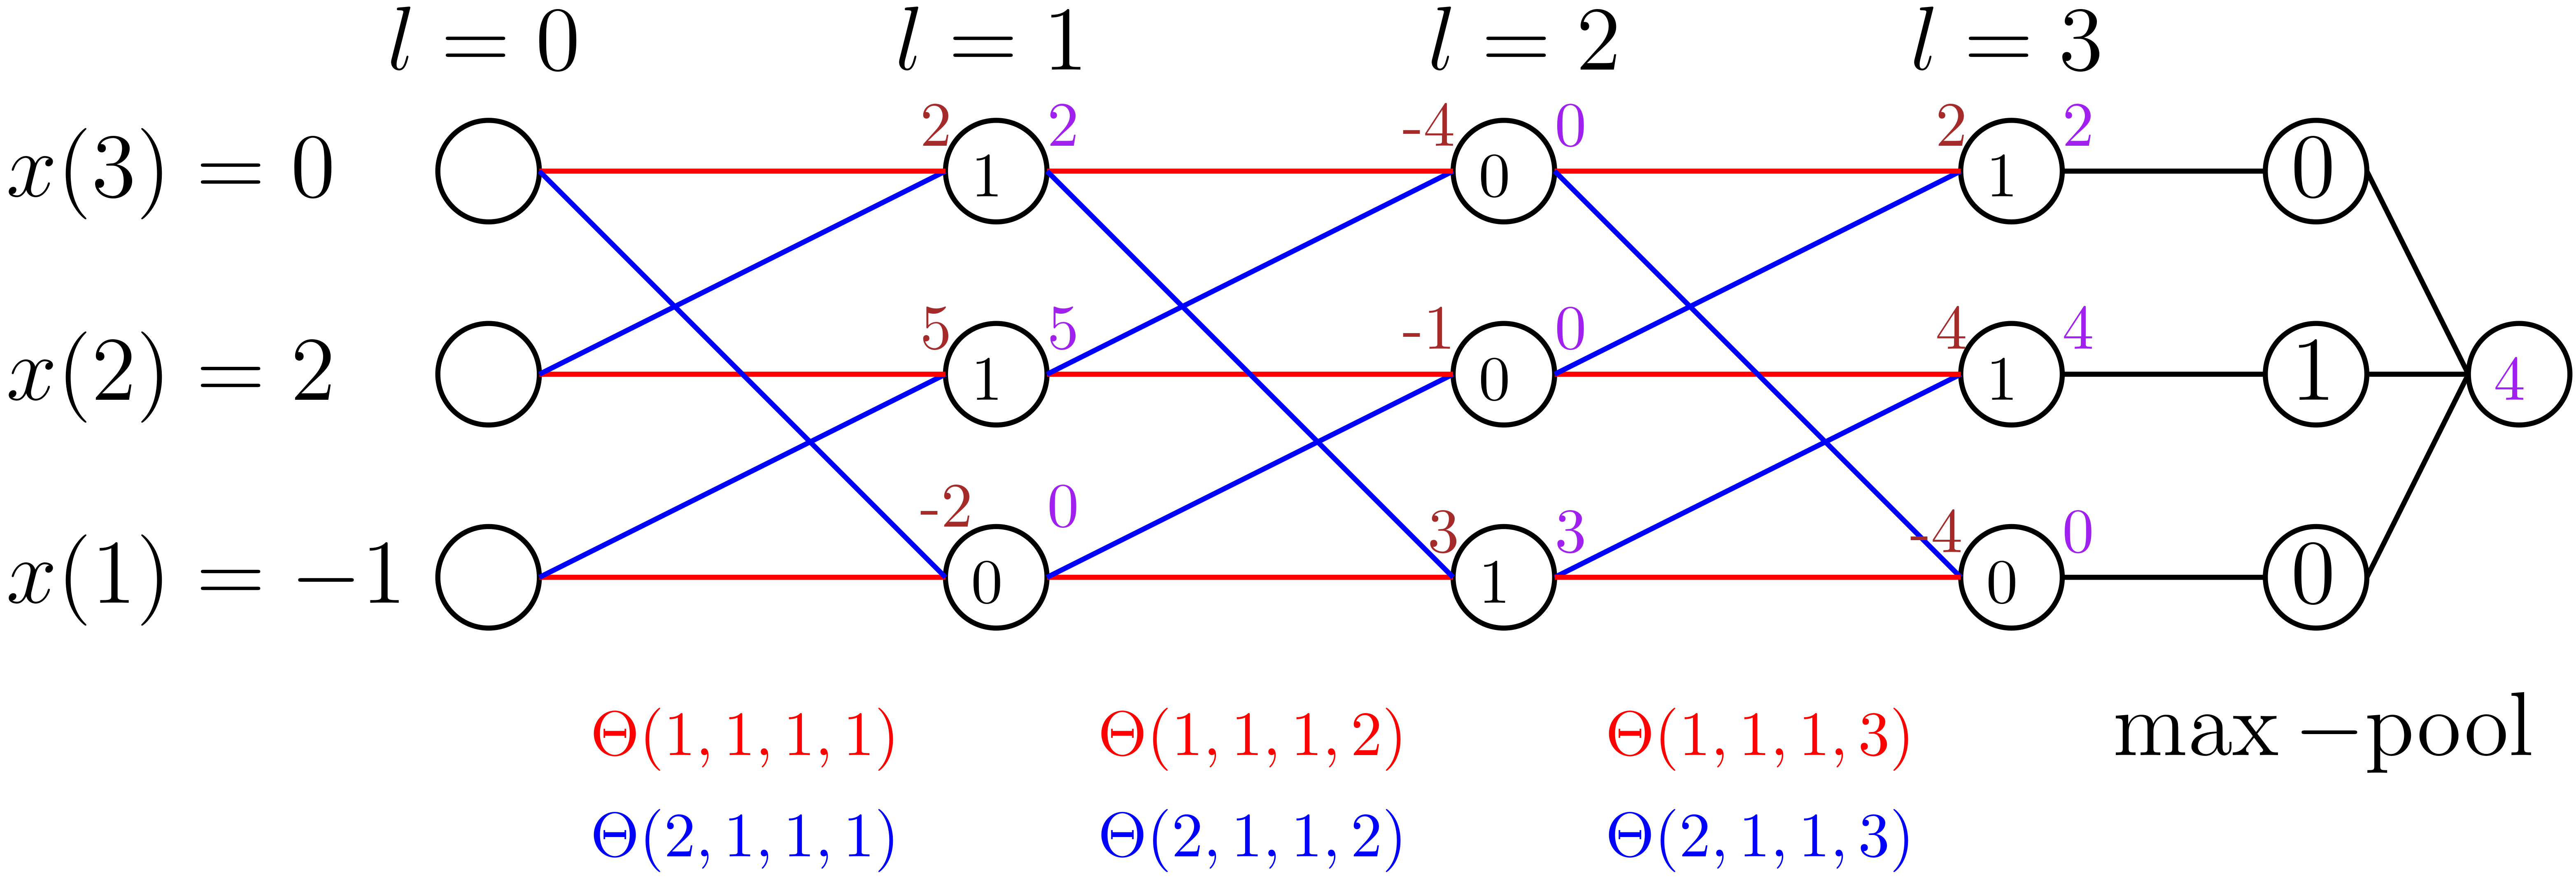
\includegraphics[angle=0.2,scale=0.1]{figs/maxp2.png}
}
\end{minipage}
\caption{\small{Shows weight sharing and rotational symmetry of internal variables and the output after pooling in a CNN. Left most cartoon uses a GAP layer, and the other two cartoons use $\max$-pooling. Circles are nodes and the $1/0$ in the nodes indicate the gating. Pre-activations/node output are shown in {\color{chocolate}{brown}}/{\color{electricpurple}{purple}}.}}
\label{fig:pathshare}
\end{figure}
\begin{definition}[Neural Path Value]
The product of the weights and normalisation factors in a path $p$ is its `value'. The value of a path bundle is the value of any path in that bundle. The path/bundle values are denoted by $v_{\Theta}(p)/v_{\Theta}(B_{\hat{p}})$ and are defined as follows:

(a) $v_{\Theta}(p)=\Pi_{l=1}^d \Theta(\I_{l-1}(p),\I_l(p),l)$.


(b) $v_{\Theta}(B_{\hat{p}})= \Pi_{l=1}^{\dc} \Theta(\Iconv_{l}(p),\I_{l-1}(p),\I_{l}(p),l) \cdot \Pi_{l=\dc+2}^{\dc+\dfc+1} \Theta(\I_{l-1}(p),\I_l(p),l)$, for any $p\in B_{\hat{p}}$.

(c) $v_{\Theta}(p)=\Pi_{l=1}^d \Theta(\I_{l-1}(p),\I_l(p),l) \cdot \Gamma(\I^{\J}(p))$.

The neural path value is defined as $v_{\Theta}\eqdef (v_{\Theta}(p),p\in [\Pfc])\in\R^{\Pfc}$, $v_{\Theta}\eqdef (v_{\Theta}(B_{\hat{p}}),\hat{p}\in [\hat{P}^{\text{cnn}}])\in\R^{\hat{P}^{\text{cnn}}}$, and $v_{\Theta}\eqdef (v_{\Theta}(p),p\in [\Pres])\in\R^{\Pres}$ for FC-DNN, CNN and ResNet respectively.
 \end{definition}
\begin{proposition}[Rotational Invariance]\label{prop:rot}
Internal variables in the convolutional layers are circularly symmetric,  i.e., for $r\in\{0,\ldots,\din-1\}$ it follows that (i) $z_{rot(x,r),\Theta}(\ifout,\cdot,\cdot) = z_{x,\Theta}(\ifout \oplus r,\cdot,\cdot)$, (ii) $q_{rot(x,r),\Theta}(\ifout,\cdot,\cdot) = q_{x,\Theta}(\ifout \oplus r,\cdot,\cdot)$ and (iii) $G_{rot(x,r),\Theta}(\ifout,\cdot,\cdot) = G_{x,\Theta}(\ifout \oplus r,\cdot,\cdot)$.
\end{proposition}
\begin{definition}
The neural path feature (NPF) corresponding to a path $p$ is given by 

(a) $\phi_{x,\Theta}(p)\eqdef  x(\Ifeat_0(p))A_{\Theta}(x_s,p)$ for  FC-DNN and ResNet.

(b) $\phi_{x,\Theta}(\hat{p})\eqdef \sum_{\hat{p}\in B_{\hat{p}}}x(\Ifeat_0(p))A_{\Theta}(x,p)$ for CNN.

The NPF is defined as $\phi_{x,\Theta}\eqdef (\phi_{x,\Theta}(p),p\in [\Pfc])\in\R^{\Pfc}$, $\phi_{x,\Theta}\eqdef (\phi_{x,\Theta}(B_{\hat{p}}),\hat{p}\in [\hat{P}^{\text{cnn}}])\in\R^{\hat{P}^{\text{cnn}}}$, and $\phi_{x,\Theta}\eqdef (\phi_{x,\Theta}(p),p\in [\Pres])\in\R^{\Pres}$ for FC-DNN, CNN and ResNet respectively.
\end{definition}
\begin{proposition}[Output=$\langle$NPF,NPV$\rangle$]\label{prop:zero}  The output of the network can be written as an inner product of the NPF and NPV, i.e., 
$\hat{y}_{\Theta}(x)=\ip{\phi_{x,\Theta},v_{\Theta}}$.
\end{proposition}
\begin{comment}
\FloatBarrier
\begin{table}[h]
\resizebox{\columnwidth}{!}{
\begin{tabular}{|c|c|c|c|}\hline
Quantity& FC& CNN & ResNet\\\hline
%Total Paths & $\Pfc=\din w^{(d-1)}$ & $\Pcnn=\din(\wconv w)^{\dc}w^{(\dfc-1)}$ & $\Pres = \din \cdot\sum_{i=0}^b \binom{b}{i} w^{(i+2)\dblock-1}$\\\hline
%Path-per Bundle& $1$ & $\din$ &$1$\\\hline
$A_{\Theta}(x,p)$	&$\Pi_{l=1}^{d-1} G_{x,\Theta}(\I_l(p),l)$ &\shortstack{$\left(\Pi_{l=1}^{\dc} G_{x,\Theta}(\Ifeat_l(p),\Iconv_l(p),l)\right)$ \\ $\cdot \left(\Pi_{l=\dc+2}^{\dc+\dfc+1} G_{x,\Theta}(\Ifc_l(p),l)\right)$} &  $\Pi_{l=1}^{d-1} G_{x,\Theta}(\I_l(p),l)$\\\hline 
$\phi_{x,\Theta}(p)$ & $x(\I_0(p))A_{\Theta}(x_s,p)$ & $\sum_{\hat{p}\in B_{\hat{p}}}x(\Ifeat_0(p))A_{\Theta}(x,p)$ & $x(\I_0(p))A_{\Theta}(x_s,p)$\\\hline

$v_{\Theta}(p)$ & $\Pi_{l=1}^d \Theta(\I_{l-1}(p),\I_l(p),l)$ &$ v_{\Theta}(B_{\hat{p}}$ &\shortstack{$  \Pi_{l=1}^d \Theta(\I_{l-1}(p),\I_l(p),l)\cdot$\\ $\Gamma(\I^{\J}(p))$}\\\hline
\end{tabular}
}
\end{table}
\end{comment}
